
\newcommand{\insertFigCompToy}{
\begin{figure}
\centering
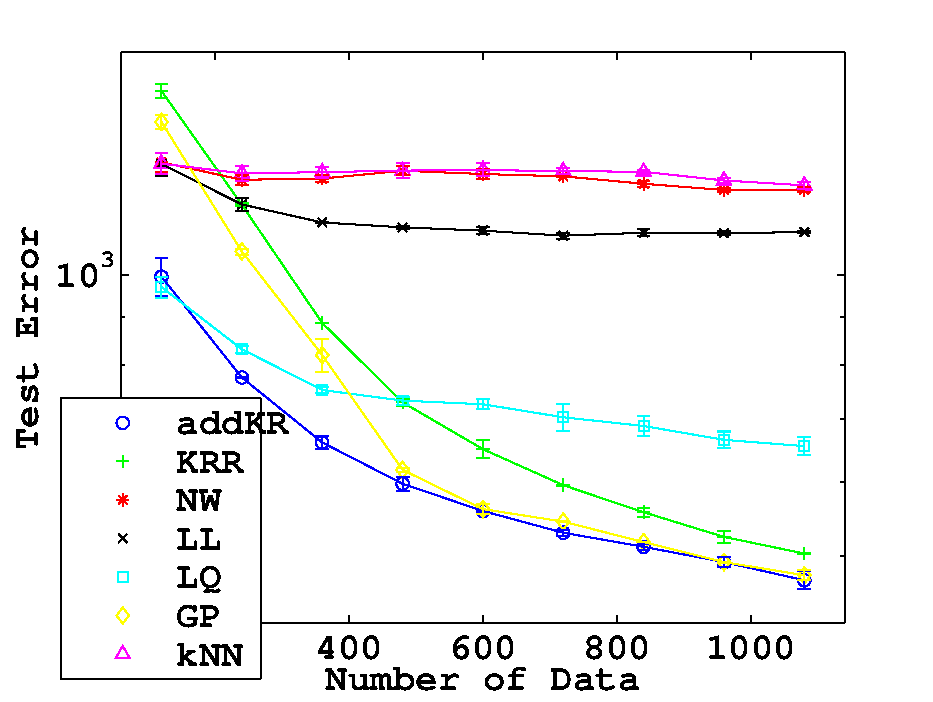
\includegraphics[width=3.2in]{figs/compToy}
\vspace{\imcaptionspace}
\caption[]{\small Comparison of various nonparametric regression methods on a
$20$-dimensional toy dataset. The $x$-axis denotes the number of training data
and the $y$-axis is the test error. }
% \vspace{\imtextspace}
\vspace{-0.2in}
\label{fig:compToy}
\end{figure}
}

\newcommand{\insertFigOpt}{
\begin{figure}
\centering
\subfigure[]{
  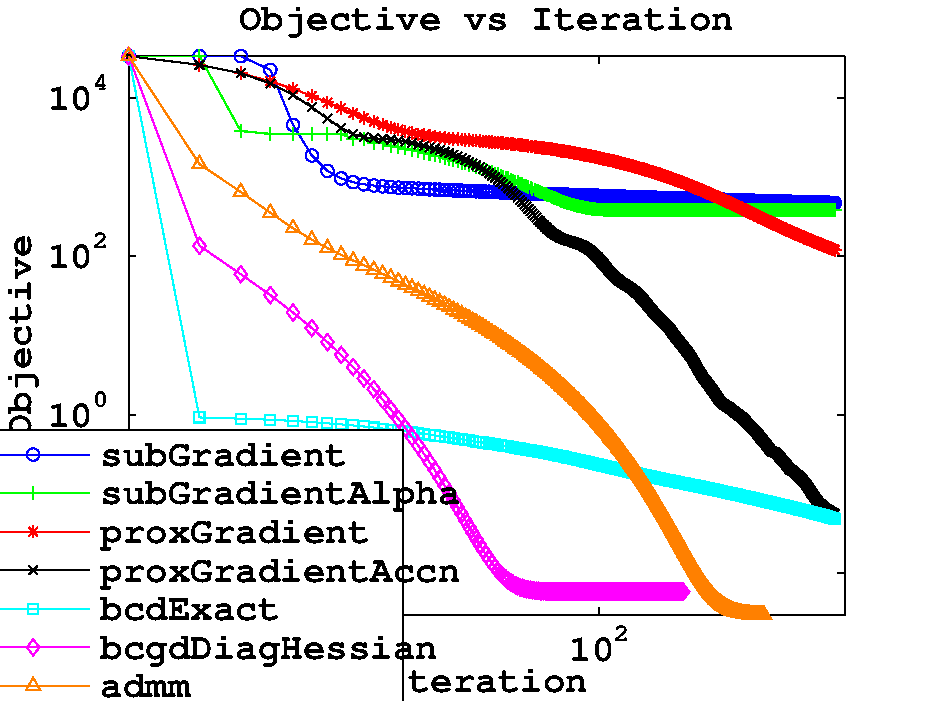
\includegraphics[width=\imarrwtwo]{figs/iteration1000v2} \hspace{\imhsptwo}
  \vspace{\imlabelspace}
  \label{fig:optCompIter}
}
\subfigure[]{
  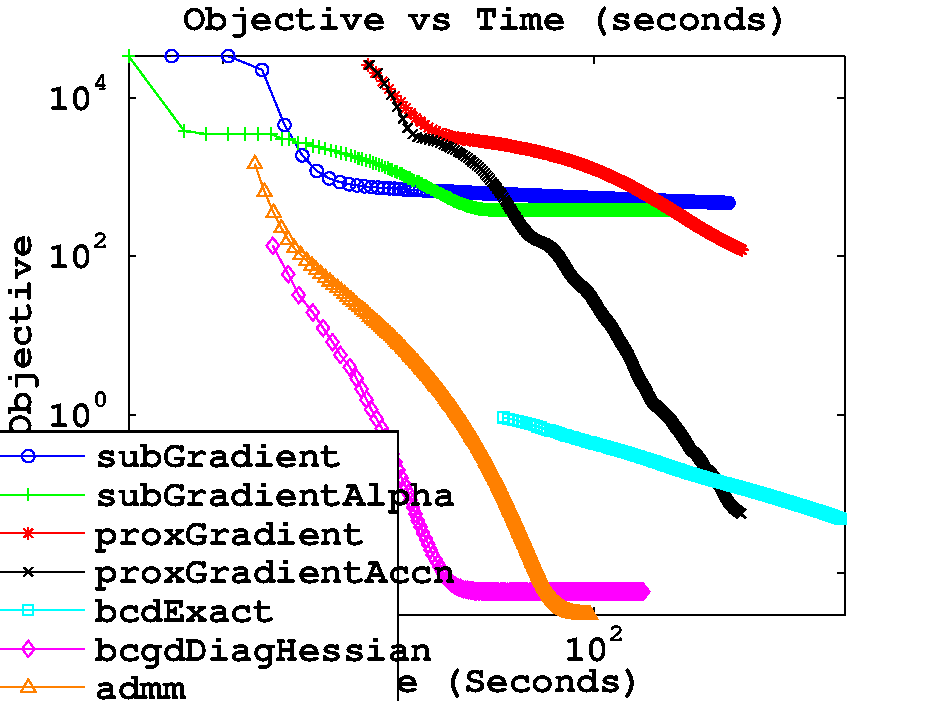
\includegraphics[width=\imarrwtwo]{figs/time1000v2} \hspace{\imhsptwo}
  \vspace{\imlabelspace}
  \label{fig:optCompTime}
}
\caption[]{\small
\subref{fig:optCompIter}: Comparison of the different methods to optimise our
objective. In~\subref{fig:optCompIter} The $x$-axis is the iteration and
in~\subref{fig:optCompTime} the $x$-axis is time. In both figures
 the $y$-axis is the objective. 
Both figures are in log-log scale.
}
% \vspace{-0.2in}
\label{fig:opt}
\end{figure}
}

\newcommand{\insertFigRegFSel}{
\begin{figure}
\centering
\subfigure[]{
  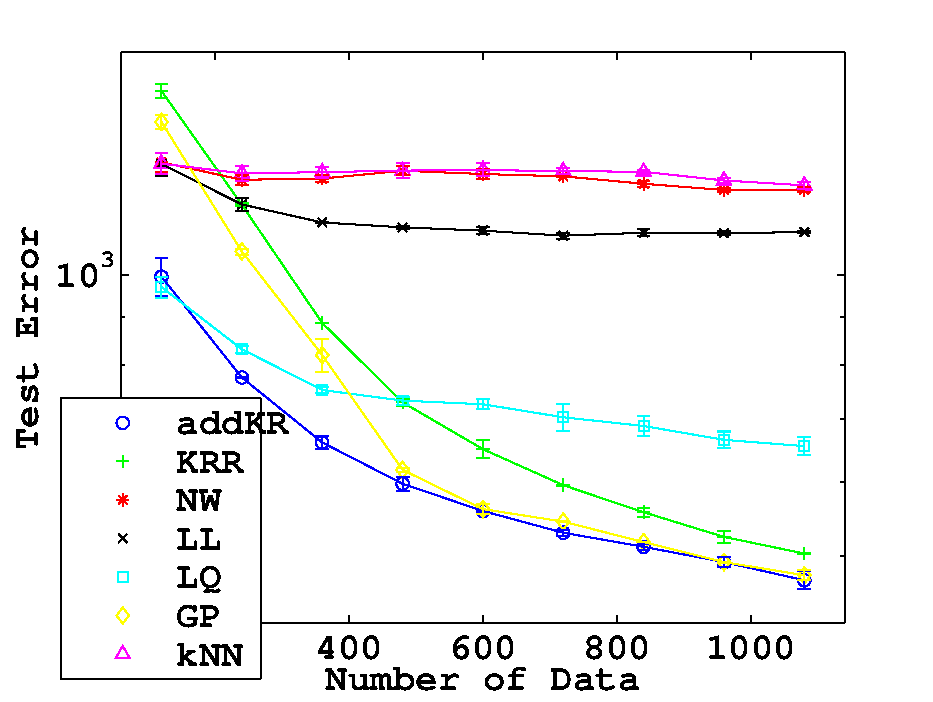
\includegraphics[width=\imarrwtwo]{figs/compToy} \hspace{\imhsptwo}
  \vspace{\imlabelspace}
  \label{fig:compToy}
} \\
\vspace{-0.1in}
\subfigure[]{
  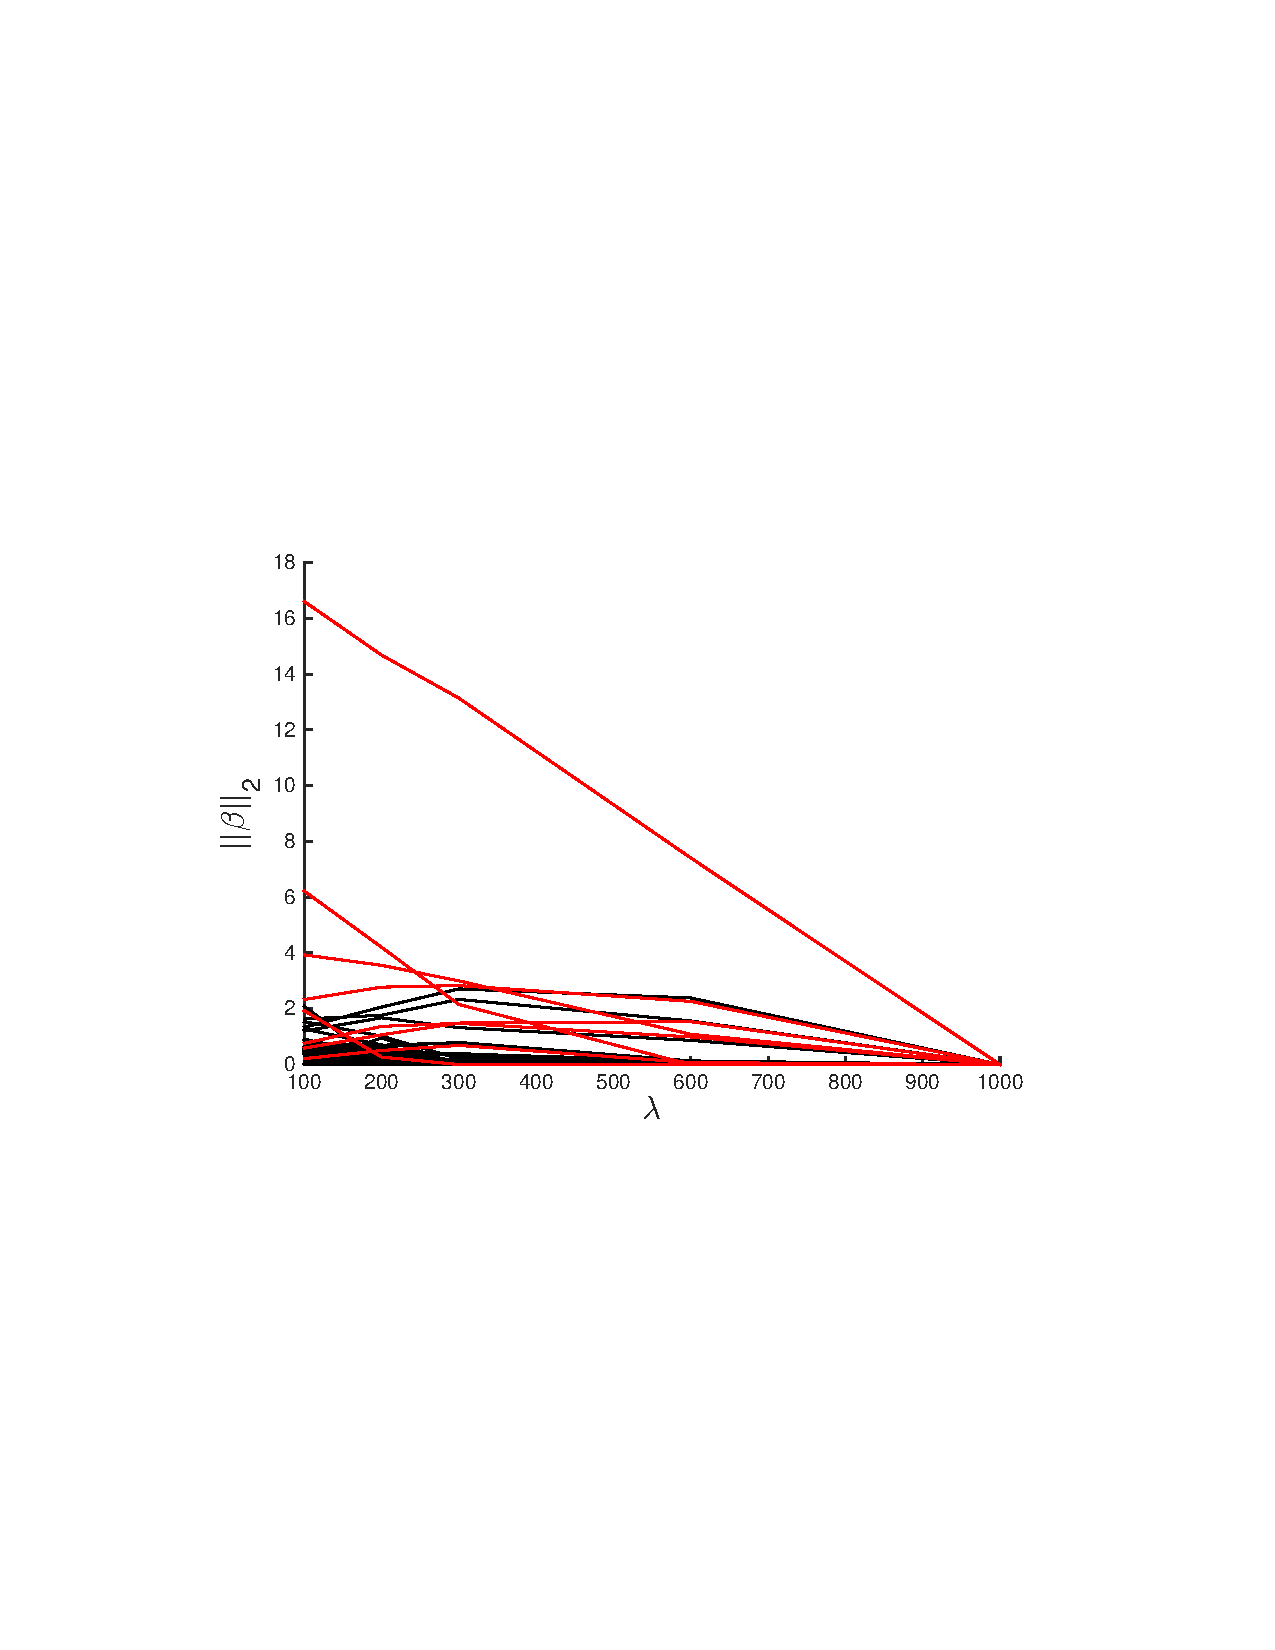
\includegraphics[width=\imarrwtwo]{figs/solnpath600} \hspace{\imhsptwo}
  \vspace{\imlabelspace}
  \label{fig:solnpath}
}
\caption[]{\small
\subref{fig:compToy}: Comparison of \addkrrs using ESP Kernels against other 
nonparametric methods
on a $20$ dimensional toy problem. The $x$-axis denotes the number of training
points and the $y$-axis is the error on a test set.
\subref{fig:solnpath}: Solution path with $n=600$ samples for the synthetic
problem. The $x$-axis shows the regularisation parameter while the $y$-axis
plots $\|\funcj\|_{\Hcalkj} = \|\betaj\|$. The true nonzero functions are
depicted in red. 
% As the figure indicates several of the false functions are
% driven to $0$ fast whereas the true functions persist for longer.
}
% \vspace{-0.2in}
\end{figure}
}



\newcommand{\insertFigSolnPath}{
\begin{figure}
\centering
% 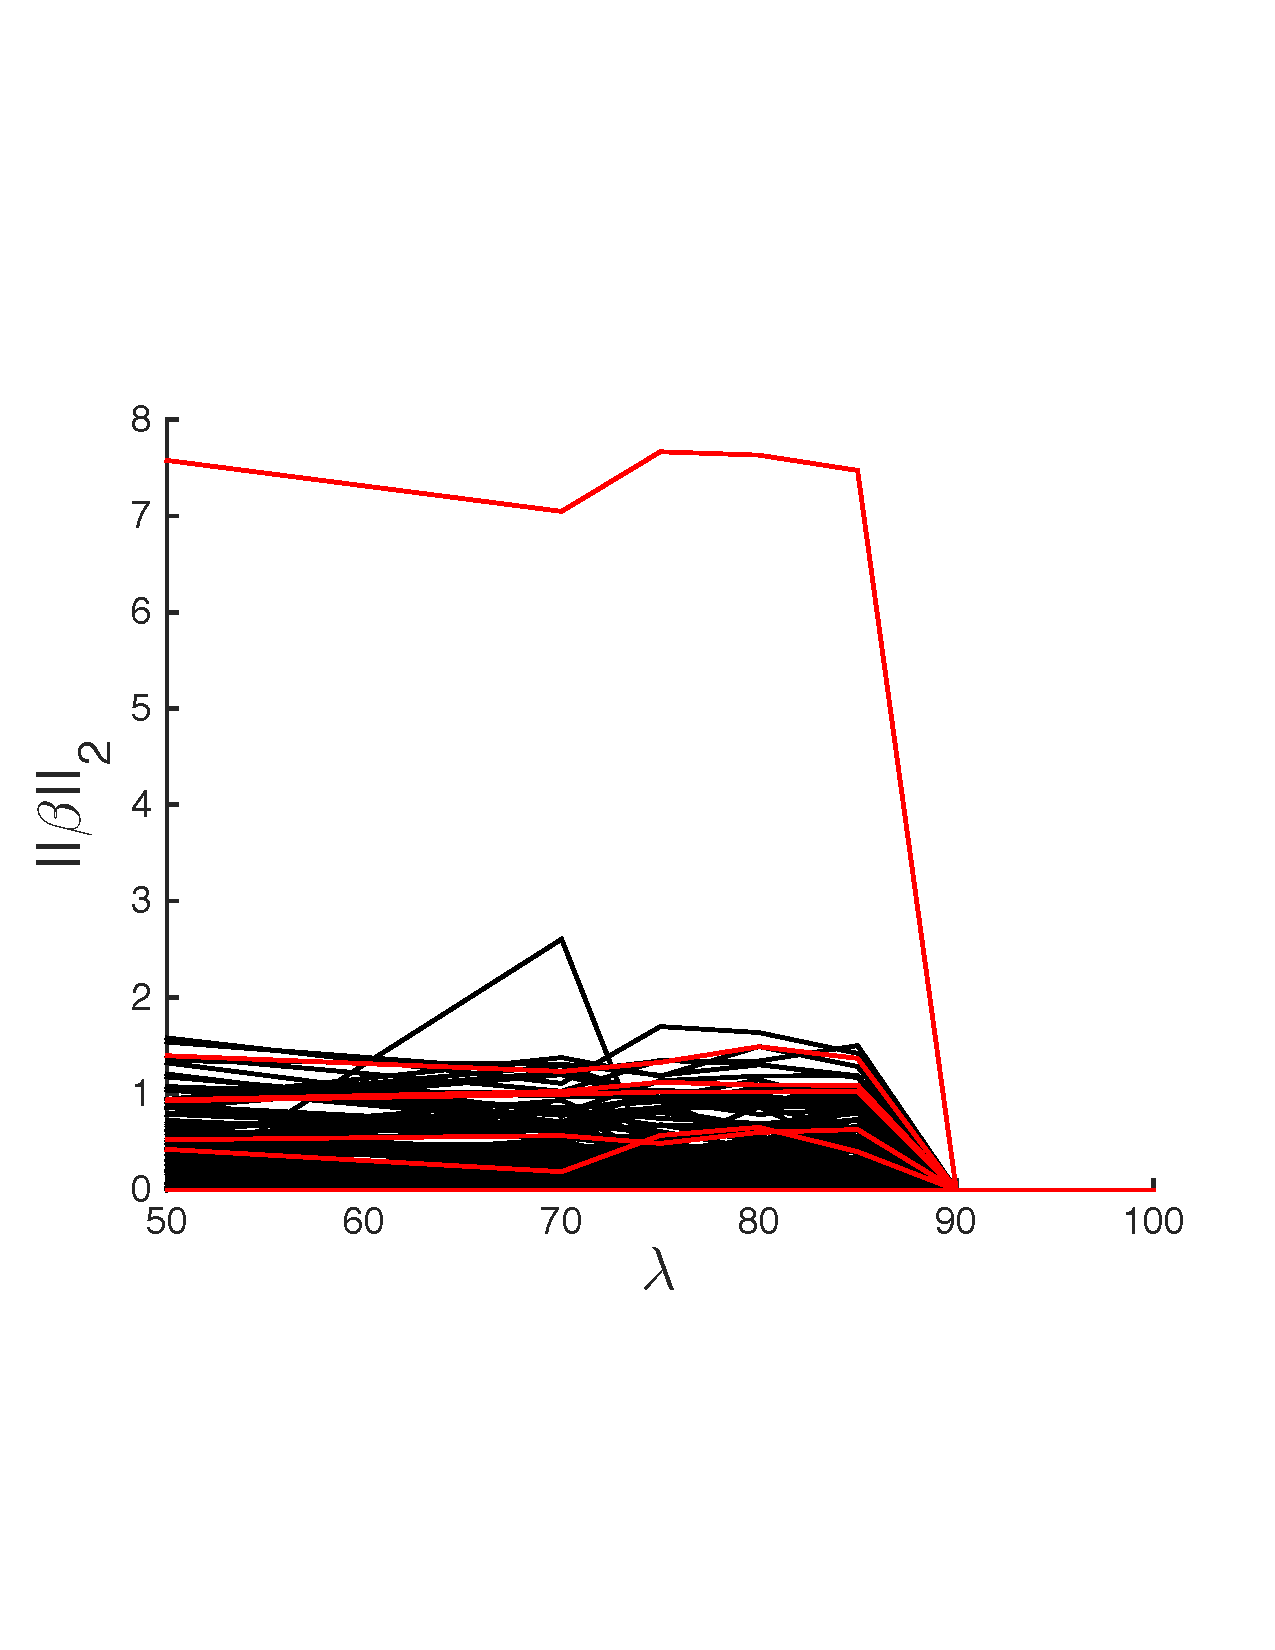
\includegraphics[width=3.4in]{figs/solnpath200.pdf}
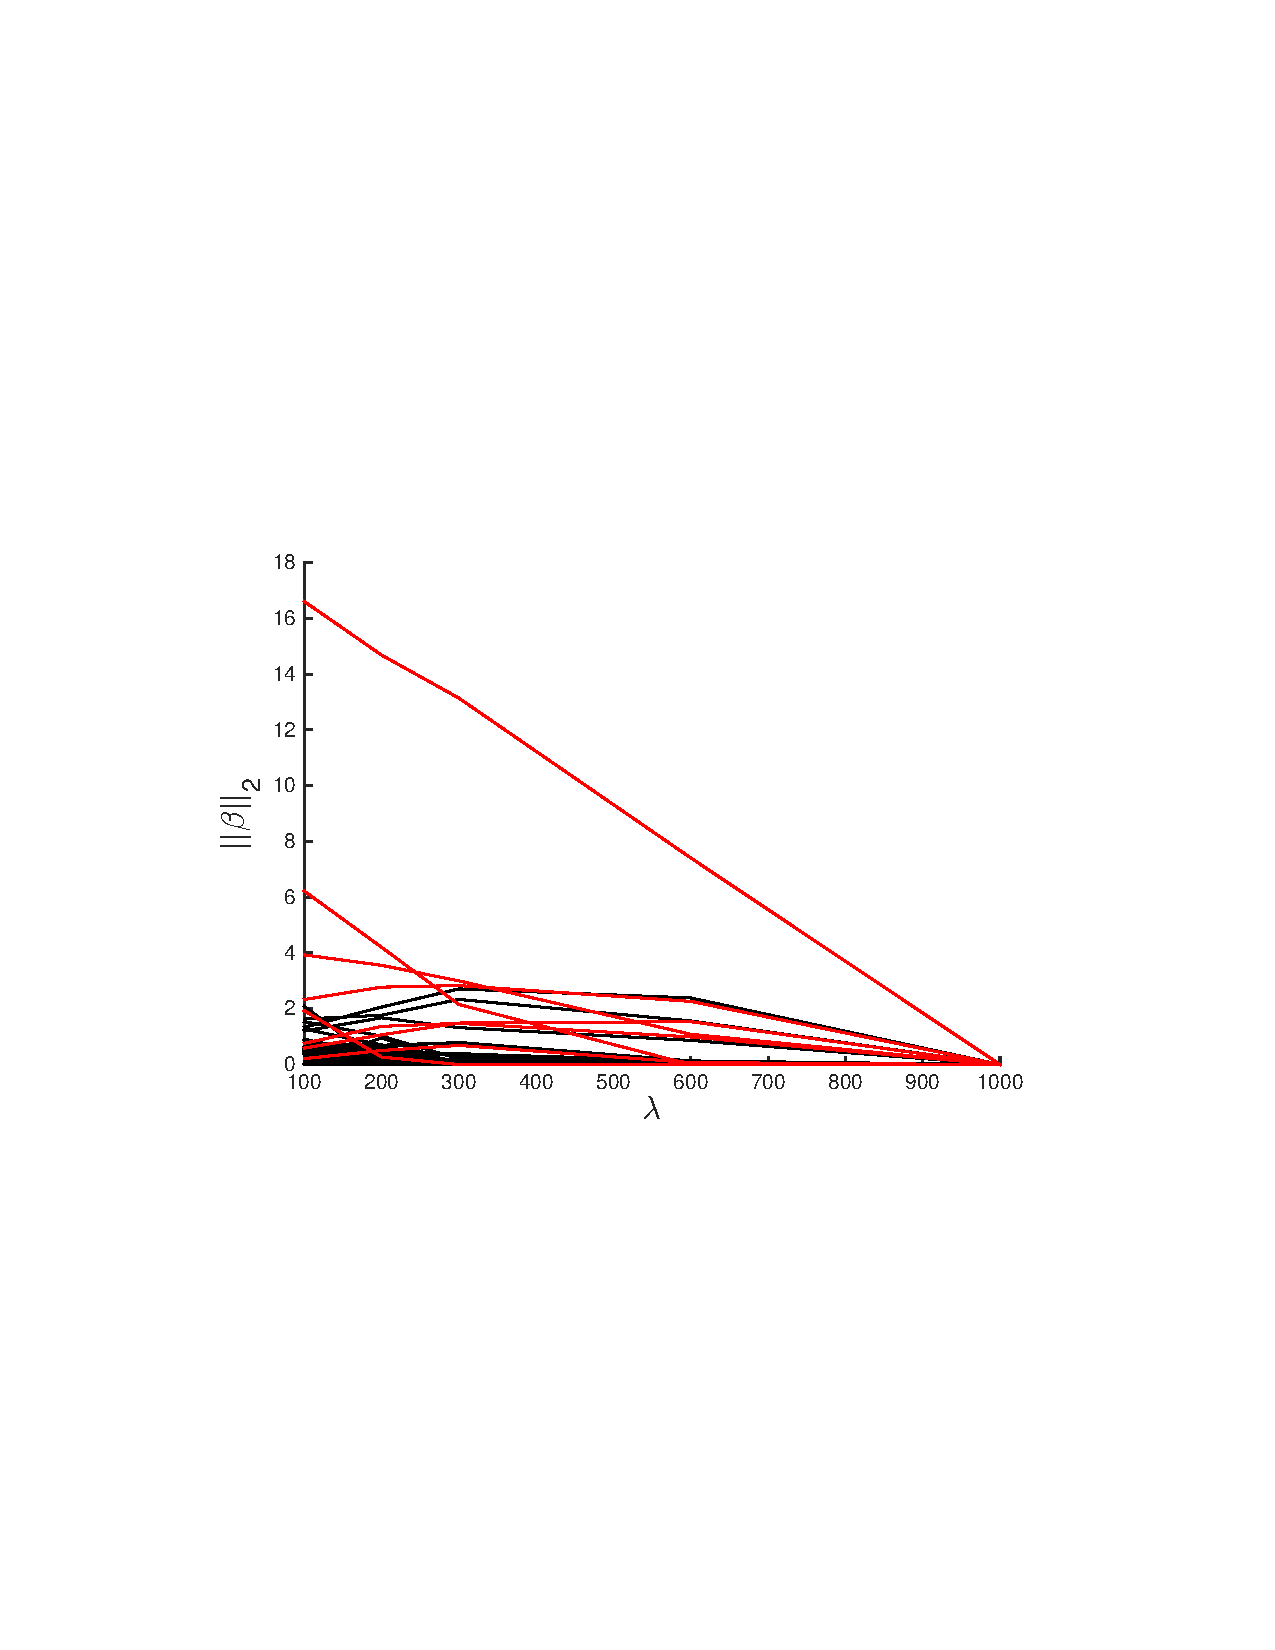
\includegraphics[width=3.2in]{figs/solnpath600.pdf}
\vspace{\imcaptionspace}
\caption[]{\small Solution path with $n=200$ samples (above) and
$n=600$ (below). The $x$-axis shows the regularization parameter,
while the $y$-axis plots $\|\funcj\|_{\Hcalkj} = \|\betaj\|$. 
The true nonzero functiosn are depicted in red. As the figure indicates, several
of the false functions are driven to $0$ fast whereas the true functions
persist for longer.
}
\vspace{\imtextspace}
\label{fig:n200}
\end{figure}
}
